%!TEX root = ../../thesis.tex

\Wjets events contribute to the background when a jet is misidentified as a lepton, and 
dijet events contribute when two jets are misidentified as leptons. This is due to leptonic 
decays of heavy flavour hadrons, hadronic showers mimicking the electromagnetic showers, or 
punchthrough into the muon spectrometer. Although the fake rates are very low, these 
backgrounds are significant because the \Wjets and dijet cross sections are many orders of 
magnitude larger than those of Higgs boson production. Since these fake rates are sensitive 
to effects that are difficult to accurately model (such as jet flavour composition, jet 
substructure and hadronic shower shapes), a data-driven \textit{fake factor method} is used 
to estimate these backgrounds.

As these two backgrounds have large uncertainties, their suppression is critically 
important. The electron and muon selection criteria are chosen to be tighter at low \pt 
(see \Section~\ref{sec:objects}), in order to reduce the fake rates where these backgrounds 
are largest. The dijet background is additionally rejected by requiring significant \met 
and by the \unit{$\maxmtw > 50$}{\GeV} cut in the 1-jet bin of the \emch/\mech channels.



\subsection{The fake factor method}
\label{sec:wjets:fakefactor_method}

The fake factor method defines two new objects: anti-identified electrons \antiid{\Pe} and 
muons \antiid{\Pmu}, collectively known as anti-identified leptons \antiid{\Plepton}. 
Loosened selection criteria ensure they are highly contaminated by jets, while a veto on 
identified leptons \id{\Plepton} removes overlap between \id{\Plepton} and \antiid{\Plepton}
objects (see \Section~\ref{sec:wjets:antiid}). The fake factor $f_{\Plepton}$ is then 
defined as the ratio of efficiencies (\ie fake rates) for jets passing the \id{\Plepton} 
criteria to passing the \antiid{\Plepton} criteria.

In the following discussion, a \textit{sample} shall refer to a collection of events 
featuring a specific set of objects, \eg the signal sample 
$\mathcal{N}_{\id{\Plepton}\id{\Plepton}\text{,OS}}$ refers to \id{\Plepton}\id{\Plepton} 
events with opposite-sign charges (the \HWW analysis uses three signal samples: 
\id{\Plepton}\id{\Plepton} = \eech{}+\mmch, \emch and \mech). A \textit{region} shall refer 
to events whose objects satisfy a set of criteria (also known as cuts), \eg the signal 
region refers to events passing the criteria in \Table~\ref{tab:event_selection}.

A dilepton sample $\mathcal{N}_{\id{\Plepton}\id{\Plepton}}$, a \Wjets control sample 
$\mathcal{N}_{\id{\Plepton}\antiid{\Plepton}}$ and a dijet control sample 
$\mathcal{N}_{\antiid{\Plepton}\antiid{\Plepton}}$ are defined, each with opposite-sign 
(OS) and same-sign (SS) charge variants. Note that $\mathcal{N}$ indicates a sample to 
which cuts may be applied, and an \antiid{\Plepton} is treated as an \id{\Plepton} in such 
cuts when appropriate. Each sample has contributions from \Wjets and dijet events, and 
events with prompt leptons from the hard scatter or photon conversions (labelled EW):
\begin{equation}
	\mathcal{N}_{\id{\Plepton}\id{\Plepton},i} &= \mathcal{N}_{\id{\Plepton}\id{\Plepton},i}^{\text{\Wjets}} + \mathcal{N}_{\id{\Plepton}\id{\Plepton},i}^{\text{dijet}} + \mathcal{N}_{\id{\Plepton}\id{\Plepton},i}^{\text{EW}} \\
	\mathcal{N}_{\id{\Plepton}\antiid{\Plepton},i} &= \mathcal{N}_{\id{\Plepton}\antiid{\Plepton},i}^{\text{\Wjets}} + \mathcal{N}_{\id{\Plepton}\antiid{\Plepton},i}^{\text{dijet}} + \mathcal{N}_{\id{\Plepton}\antiid{\Plepton},i}^{\text{EW}} \\
	\mathcal{N}_{\antiid{\Plepton}\antiid{\Plepton},i} &= \mathcal{N}_{\antiid{\Plepton}\antiid{\Plepton},i}^{\text{\Wjets}} + \mathcal{N}_{\antiid{\Plepton}\antiid{\Plepton},i}^{\text{dijet}} + \mathcal{N}_{\antiid{\Plepton}\antiid{\Plepton},i}^{\text{EW}}
\end{equation}
where $i = \text{OS, SS}$. $\mathcal{N}_{\id{\Plepton}\id{\Plepton},i}$ is dominated by 
$\mathcal{N}_{\id{\Plepton}\id{\Plepton},i}^{\text{EW}}$, 
$\mathcal{N}_{\id{\Plepton}\antiid{\Plepton},i}$ is dominated by 
$\mathcal{N}_{\id{\Plepton}\antiid{\Plepton},i}^{\text{\Wjets}}$ and 
$\mathcal{N}_{\antiid{\Plepton}\antiid{\Plepton},i}$ is dominated by 
$\mathcal{N}_{\antiid{\Plepton}\antiid{\Plepton},i}^{\text{dijet}}$. 

The purpose of the fake factor method is to estimate the 
$\mathcal{N}_{\id{\Plepton}\id{\Plepton}\text{,OS}}^{\text{\Wjets}}$ and 
$\mathcal{N}_{\id{\Plepton}\id{\Plepton}\text{,OS}}^{\text{dijet}}$ contributions to the 
$\mathcal{N}_{\id{\Plepton}\id{\Plepton}\text{,OS}}$ signal sample. The SS versions are 
required in the non-\WW diboson background estimation (see \Section~\ref{sec:diboson}). It 
does this in a data-driven way by using the \Wjets and dijet control samples, subtracting 
the expected contaminations, and then multiplying by a data-driven fake factor 
$f_{\Plepton}$ (defined earlier):
\begin{equation}
	\mathcal{N}_{\id{\Plepton}\id{\Plepton},i}^{\text{pred,dijet}} &= \parenths{\mathcal{N}_{\antiid{\Plepton}\antiid{\Plepton},i}^{\text{data}} - \mathcal{N}_{\antiid{\Plepton}\antiid{\Plepton},i}^{\text{MC,\Wjets}} - \mathcal{N}_{\antiid{\Plepton}\antiid{\Plepton},i}^{\text{MC,EW}}} \cdot f_{\Plepton \vert \antiid{\Plepton}}^{\text{pred,dijet}} \cdot f_{\Plepton \vert \id{\Plepton}}^{\text{pred,dijet}} \label{eq:dijet_bkgto_dilepton} \\
	\mathcal{N}_{\id{\Plepton}\antiid{\Plepton},i}^{\text{pred,dijet}} &= \parenths{\mathcal{N}_{\antiid{\Plepton}\antiid{\Plepton},i}^{\text{data}} - \mathcal{N}_{\antiid{\Plepton}\antiid{\Plepton},i}^{\text{MC,\Wjets}} - \mathcal{N}_{\antiid{\Plepton}\antiid{\Plepton},i}^{\text{MC,EW}}} \cdot \!\sum\limits_{\antiid{\Plepton}} f_{\Plepton \vert \antiid{\Plepton}}^{\text{pred,dijet}} \label{eq:dijet_bkgto_wjet} \\
	\mathcal{N}_{\id{\Plepton}\id{\Plepton},i}^{\text{pred,\Wjets}} &= \parenths{\mathcal{N}_{\id{\Plepton}\antiid{\Plepton},i}^{\text{data}} - \mathcal{N}_{\id{\Plepton}\antiid{\Plepton},i}^{\text{pred,dijet}} - \mathcal{N}_{\id{\Plepton}\antiid{\Plepton},i}^{\text{MC,EW}}} \cdot f_{\Plepton,i}^{\text{pred,\Wjets}} \label{eq:wjet_bkgto_dilepton}
\end{equation}
where $i = \text{OS, SS}$. In the \emch/\mech channels, there are in fact two terms because 
an electron or a muon could be the fake. The dijet contamination to the \Wjets control 
sample $\mathcal{N}_{\id{\Plepton}\antiid{\Plepton},i}^{\text{pred,dijet}}$ is data-driven 
from the dijet control sample. As discussed later, the fake factors are determined by the 
flavour composition of the jets, and thus depend upon the process. Also, 
$f_{\Plepton}^{\text{pred,dijet}}$ depends upon whether the other object in the event is 
an ID lepton ($f_{\Plepton \vert \id{\Plepton}}^{\text{pred,dijet}}$) or an anti-ID 
lepton ($f_{\Plepton \vert \antiid{\Plepton}}^{\text{pred,dijet}}$). This shall be 
discussed in \Section~\ref{sec:wjets:dijet_bkg}. Finally, note that 
$f_{\Plepton}^{\text{pred,\Wjets}}$ depends upon whether the event is OS or SS. This 
shall be discussed in \Section~\ref{sec:wjets:wjet_bkg}.

An advantage of this sample-based fake factor method compared to that used in the \WW cross 
section measurement (see \Section~\ref{sec:ww:bkg}) is that it provides a background 
estimation in regions other than the signal region.

The rest of this section on the \Wjets and dijet backgrounds shall be spent describing 
the anti-identification lepton selection criteria (\Section~\ref{sec:wjets:antiid}), the 
measurement of fake factors in experimental data (Sections~\ref{sec:wjets:dijet_ff} and 
\ref{sec:wjets:zjet_ff}), and MC-based corrections to these fake factors to improve the 
background estimations (Sections~\ref{sec:wjets:wjet_bkg} and \ref{sec:wjets:dijet_bkg}).



\subsection{Lepton anti-identification criteria}
\label{sec:wjets:antiid}

The \antiid{\Plepton} selection criteria are loosened with respect to the \id{\Plepton} 
selection criteria in order to accept more jets. An explicit veto upon \id{\Plepton} objects 
avoids overlap between samples.

Relative to the \id{\Pe} definition in \Section~\ref{sec:objects:electrons}, anti-ID 
electrons of any \pt must fail the \textit{medium} identification criteria (though instead 
must have $n_{\text{pixel}}^{\text{hit}} + n_{\text{SCT}}^{\text{hit}} \geq 4$). Also, the 
tracker and calorimeter isolation are loosened to $\ptcone{0.3}/\et < 0.16$ and 
$\etcone{0.3}/\et < 0.30$.

Relative to the \id{\Pmu} definition in \Section~\ref{sec:objects:muons}, anti-ID muons have 
their transverse impact parameter $d_0$ requirement removed. Also, the tracker isolation is 
removed and the calorimeter isolation is loosened to $\etcone{0.3}/\pt < 0.15$ for 
\unit{$\pt \in \hardrange{10,15}$}{\GeV}, $\etcone{0.3}/\pt < 0.25$ for 
\unit{$\pt \in \hardrange{15,20}$}{\GeV} and $\etcone{0.3}/\pt < 0.30$ for 
\unit{$\pt > 20$}{\GeV}.



\subsection{Dijet fake factor measurement}
\label{sec:wjets:dijet_ff}

\textit{In situ} fake factor measurements are made using dijet events. This involves 
counting the numbers of \id{\Plepton} and \antiid{\Plepton} objects in a dijet control 
region (CR), subtracting the expected contamination of prompt leptons from \PW and \PZ boson 
events, and calculating the ratio $f_{\Plepton}=N_{\id{\Plepton}}/N_{\antiid{\Plepton}}$. 
$f_{\Plepton}^{\text{data,dijet}}$ is measured as a function of \pt and $\eta$.

Following data quality requirements, events are selected using very loose (no isolation 
or electron identification criteria), but highly prescaled, lepton triggers. To reduce 
the effects of prescaling, different triggers were used for different \pt ranges, and a 
trigger containing electron identification criteria was added to aid measurement of 
$N_{\id{\Plepton}}$. 
In the $f_{\Pe}$ measurement, the \verb|EF_e5_etcut| (\unit{0.012}{\invpb}) and 
\verb|EF_e5_medium1| (\unit{0.24}{\invpb}) triggers were used for \unit{$\pt < 20$}{\GeV} 
and the \verb|EF_g24_etcut| (\unit{2.1}{\invpb}) trigger was used for 
\unit{$\pt > 24$}{\GeV}. 
In the $f_{\Pmu}$ measurement, the \verb|EF_mu6| (\unit{0.94}{\invpb}) trigger was used 
for \unit{$\pt < 15$}{\GeV} and the \verb|EF_mu15| (\unit{23}{\invpb}) trigger was used 
for \unit{$\pt > 15$}{\GeV}. The trigger naming scheme is explained in the caption of 
\Table~\ref{tab:sel:triggers}.

The dijet CR requires events to have a jet with \unit{$\pt > 15$}{\GeV} (see 
\Section~\ref{sec:objects:jets} for jet selection) balancing the triggered lepton object,
$\Delta\phi\parenths{\Plepton,j} > 0.7$. To suppress contamination from \PW boson events we 
require \unit{$\mtw < 30$}{\GeV}, and to suppress the \PZ boson background we veto events 
with a lepton pair satisfying \unit{$\mods{\mll - \mZ} < 13$}{\GeV}. Note that these 
criteria apply to both \id{\Plepton} and \antiid{\Plepton} objects. Normalisation factors 
for the MC predictions of the residual \PW and \PZ boson backgrounds are derived by 
inverting the corresponding veto.

The measured electron and muon fake factors are shown in \Figure~\ref{fig:wjets:ff_data}. 
The uncertainty is dominated by uncertainties in the subtracted electroweak contamination 
(which is conservatively scaled up and down by 20\%). $f_{\Plepton}^{\text{data,dijet}}$ is 
used in the dijet background estimation, as described in \Section~\ref{sec:wjets:dijet_bkg}.

\begin{figure}
	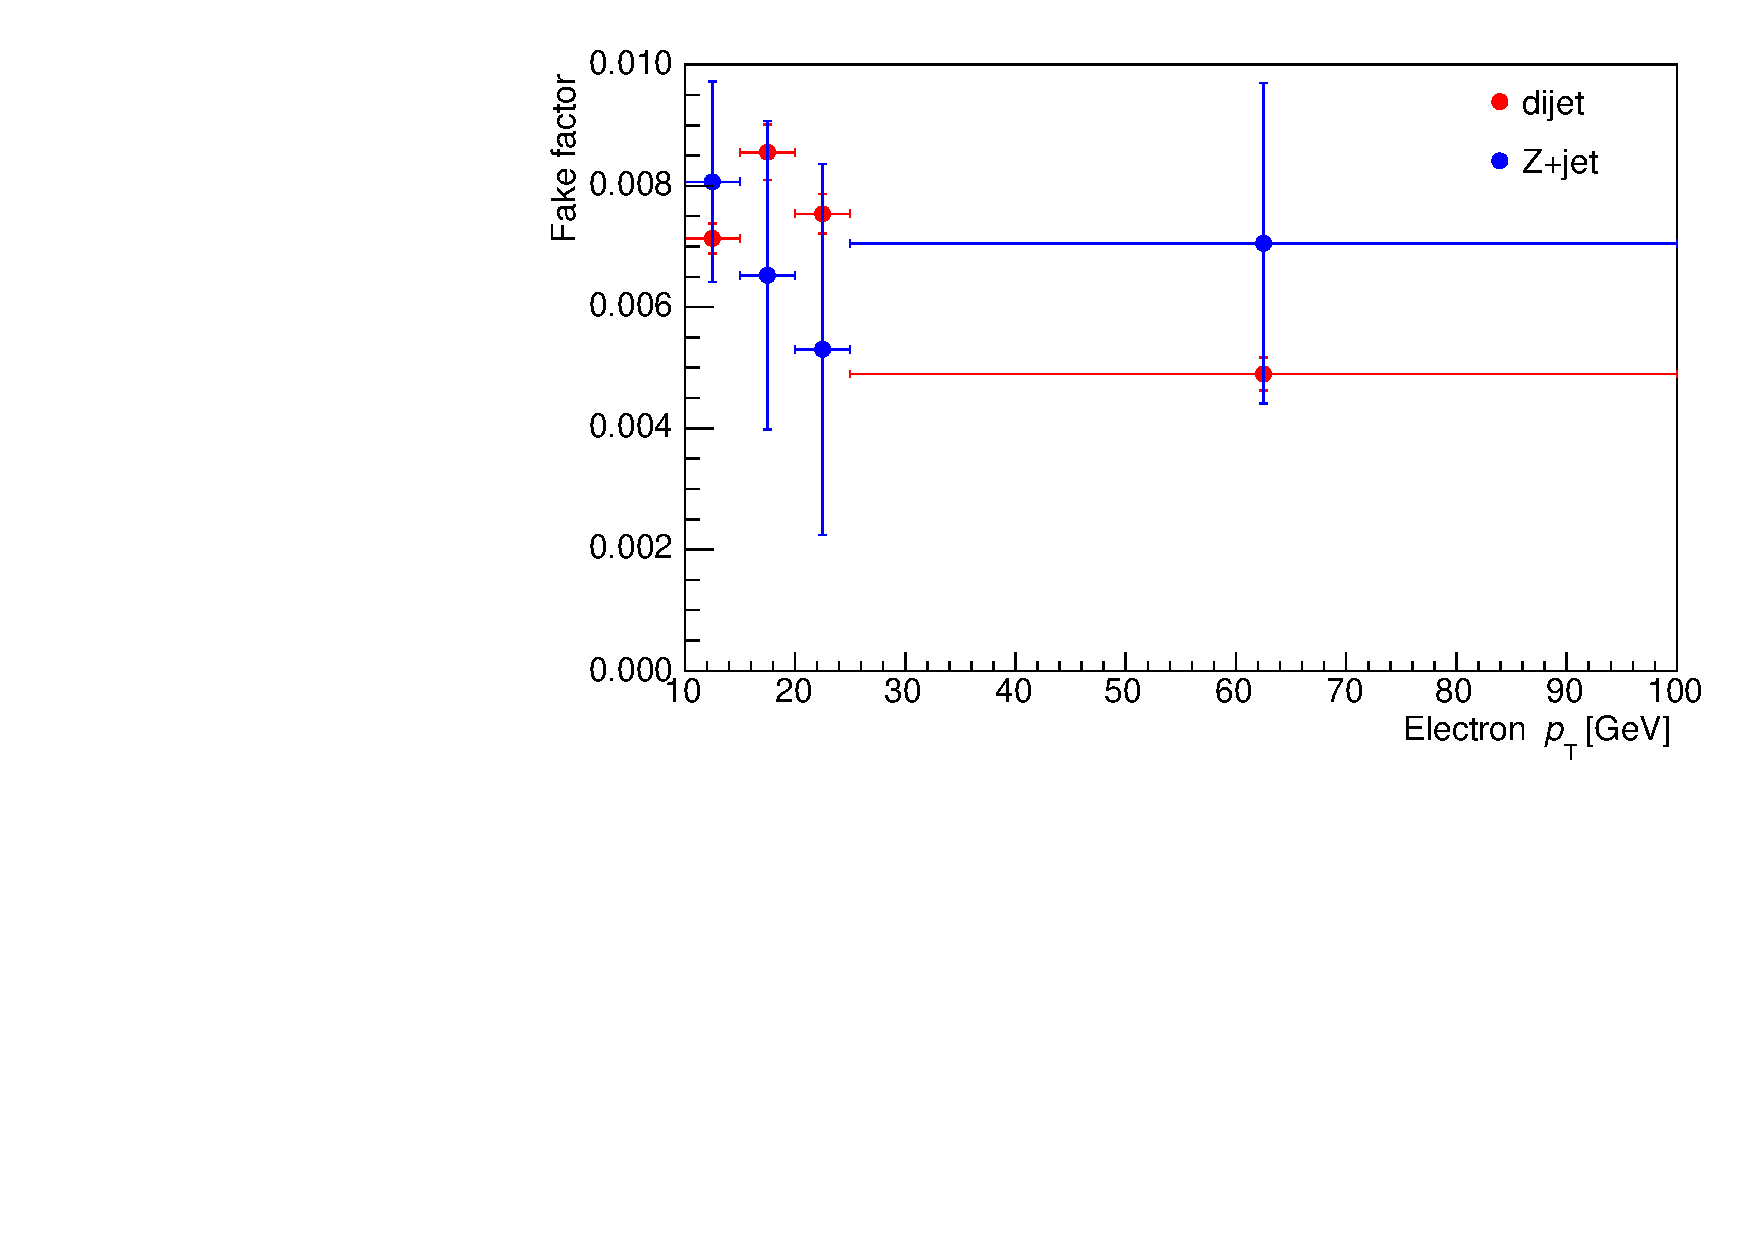
\includegraphics[width=0.495\textwidth]{custom_images/wjets/ff_el_data}
	\hfill
	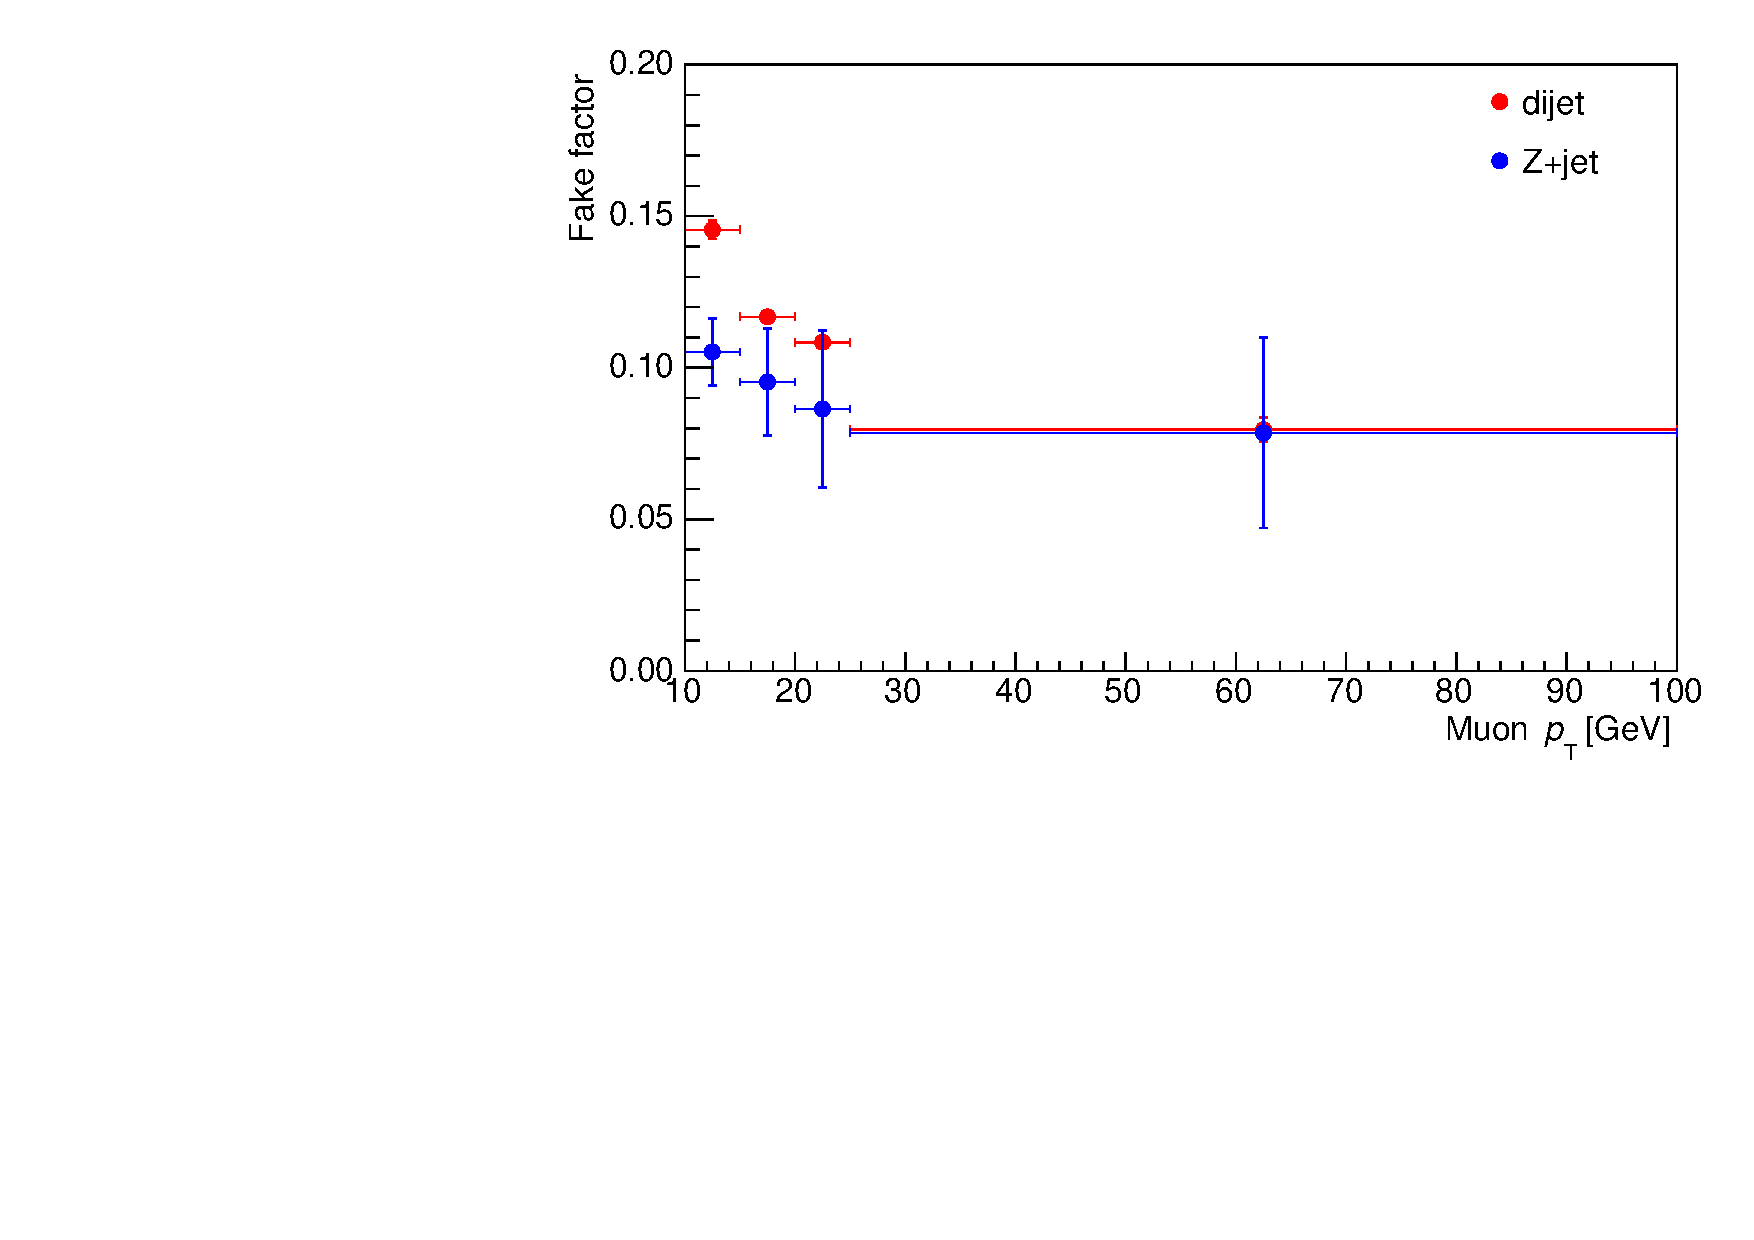
\includegraphics[width=0.495\textwidth]{custom_images/wjets/ff_mu_data}
	\caption{The fake factor measured in dijet (red) and \Zjets (blue) events versus \pt, 
	for electrons (left) and muons (right) \cite{BackgroundNote}. The error bars include 
	statistical uncertainties and uncertainties in the background subtraction.}
	\label{fig:wjets:ff_data}
\end{figure}



\subsection{\Zjets fake factor measurement}
\label{sec:wjets:zjet_ff}

\textit{In situ} fake factor measurements are also made using \Zjets events. This 
involves counting the numbers of \id{\Plepton} and \antiid{\Plepton} objects in a \Zjets 
control region (CR), subtracting the expected prompt leptons and photon conversions from 
electroweak contamination (\Zgamma, \ZZ, \Zgstar, \Wgamma, \WZ, \Wgstar), and calculating 
their ratio $f_{\Plepton} = N_{\id{\Plepton}} / N_{\antiid{\Plepton}}$.

Following data quality requirements, events are selected using unprescaled lepton 
triggers. This is possible because the triggered object is a lepton from the \PZ boson 
decay, and the \pt threshold can therefore be relatively high. In the $f_{\Pe}$ 
measurement, the \verb|EF_e24vhi_medium1| and \verb|EF_e60_medium1| triggers support 
\unit{$\pt > 25$}{\GeV}. In the $f_{\Pmu}$ measurement, the \verb|EF_mu24i_tight| and 
\verb|EF_mu36_tight| triggers are used with the dilepton \verb|EF_mu18_tight_mu8_EFFS| 
trigger to support \unit{$\pt > 22$}{\GeV}. The trigger naming scheme is explained in the 
caption of \Table~\ref{tab:sel:triggers}.

The \Zjets CR requires a pair of same-flavour and oppositely charged \id{\Plepton} objects 
to reconstruct the \PZ boson mass, \unit{$81 < \mll < 107$}{\GeV}. These leptons are 
excluded from the $f_{\Plepton}$ calculation. Electroweak contamination is suppressed by 
cuts on additional \id{\Plepton} and \antiid{\Plepton} objects: \ZZ is rejected by a veto 
on \unit{$76 < \mll < 107$}{\GeV} for additional dilepton systems, and \WZ is rejected by 
\unit{$\mtw < 30$}{\GeV}. Residual diboson backgrounds (\Zgamma, \ZZ, \Zgstar, \Wgamma, \WZ, 
\Wgstar) are subtracted using MC predictions.

The measured electron and muon fake factors are shown in \Figure~\ref{fig:wjets:ff_data}. 
The uncertainty is dominated by statistical uncertainty. For this reason, 
$f_{\Plepton}^{\text{data,\Zjets}}$ is measured as a function of \pt only, and the $\eta$ 
dependence is injected from $f_{\Plepton}^{\text{data,dijet}}$. The uncertainty due to 
electroweak subtraction is also significant (estimated by varying the diboson cross 
sections), because the contamination to the \Zjets CR is not negligible. Although 
$f_{\Plepton}^{\text{data,\Zjets}}$ has larger uncertainties than 
$f_{\Plepton}^{\text{data,dijet}}$, it shall be used in the \Wjets background estimation. 
This is because jets in \Zjets and \Wjets events are expected to have similar flavour 
composition, and therefore similar fake factors (see \Section~\ref{sec:wjets:wjet_bkg}).



\subsection{\Wjets background estimation}
\label{sec:wjets:wjet_bkg}

The \Wjets background to the opposite-sign (OS) and same-sign (SS) dilepton samples are 
estimated from the \Wjets control sample, using (\ref{eq:wjet_bkgto_dilepton}). The 
\Wjets control sample $\mathcal{N}_{\id{\Plepton}\antiid{\Plepton}}$ contains events with 
one ID lepton and one anti-ID lepton, selected from events passing the data quality 
criteria and triggers specified in \Section~\ref{sec:selection}. Generally, it is the 
lepton from the \PW boson decay that fires the single lepton triggers. Contamination is 
small, and is estimated by the fake factor method for dijet events (see 
\Section~\ref{sec:wjets:dijet_bkg}) and MC for other processes.

The fake factor of a process is determined by the jet flavour composition of that 
process. Specifically, $f_{\Pe}$ is larger for heavy flavour because the electron 
particle identification is tuned to reject light flavour jets, and $f_{\Pmu}$ is larger 
for light flavour because the $d_0$ criterion suppresses long-lived heavy flavour hadrons.

\clearpage
Since we use both OS and SS samples, it is useful to consider the jet flavour composition of 
the \Wjets process in each sample. There are diagrams like \HepProcess{\Pquark\Pgluon 
\HepTo \PW\Pquark'}, where the outgoing quark has OS charge to the \PW boson (\eg 
\HepProcess{\PW + \Pcharm}),\footnote{
	It should be emphasised that \HepProcess{\Pquark\Pgluon \HepTo \PW+\Pbottom} is highly 
	suppressed by the near unity of $V_{\Ptop\Pbottom}$	in the CKM matrix and the negligible
	top contribution to the incoming PDFs.
} 
and there are diagrams like \HepProcess{\Pquark\APquark' 
\HepTo \PW\Pgluon}, where the gluon subsequently splits to a \HepProcess{\Pquark\APquark} 
pair (\eg \HepProcess{\PW + \Pbottom\APbottom}). Therefore, in terms of the \PW and quark 
charges, the former diagrams contribute to OS only and the latter contribute to OS and 
SS equally. However, the samples are categorised according to the relative signs of the 
leptons, and so the extent to which the quark charge is preserved in the reconstructed 
lepton is important. When a hadron decays leptonically, its sign is preserved in the lepton. 
Without such a non-prompt lepton, the sign of the jet charge is more likely to be inverted 
in the reconstructed lepton. In the case of photon conversions from \HepProcess{\Ppizero 
\HepTo \Pphoton\Pphoton}, there is no asymmetry. Thus, considering the above points, there 
is a strong OS/SS asymmetry in \Pcharm-jets, a mild asymmetry in light flavour jets, and no 
asymmetry in \Pbottom-jets and \HepProcess{\Ppizero \HepTo \Pphoton\Pphoton} (see 
\Figure~\ref{fig:wjets:flav_comp}).

\begin{figure}[t]
	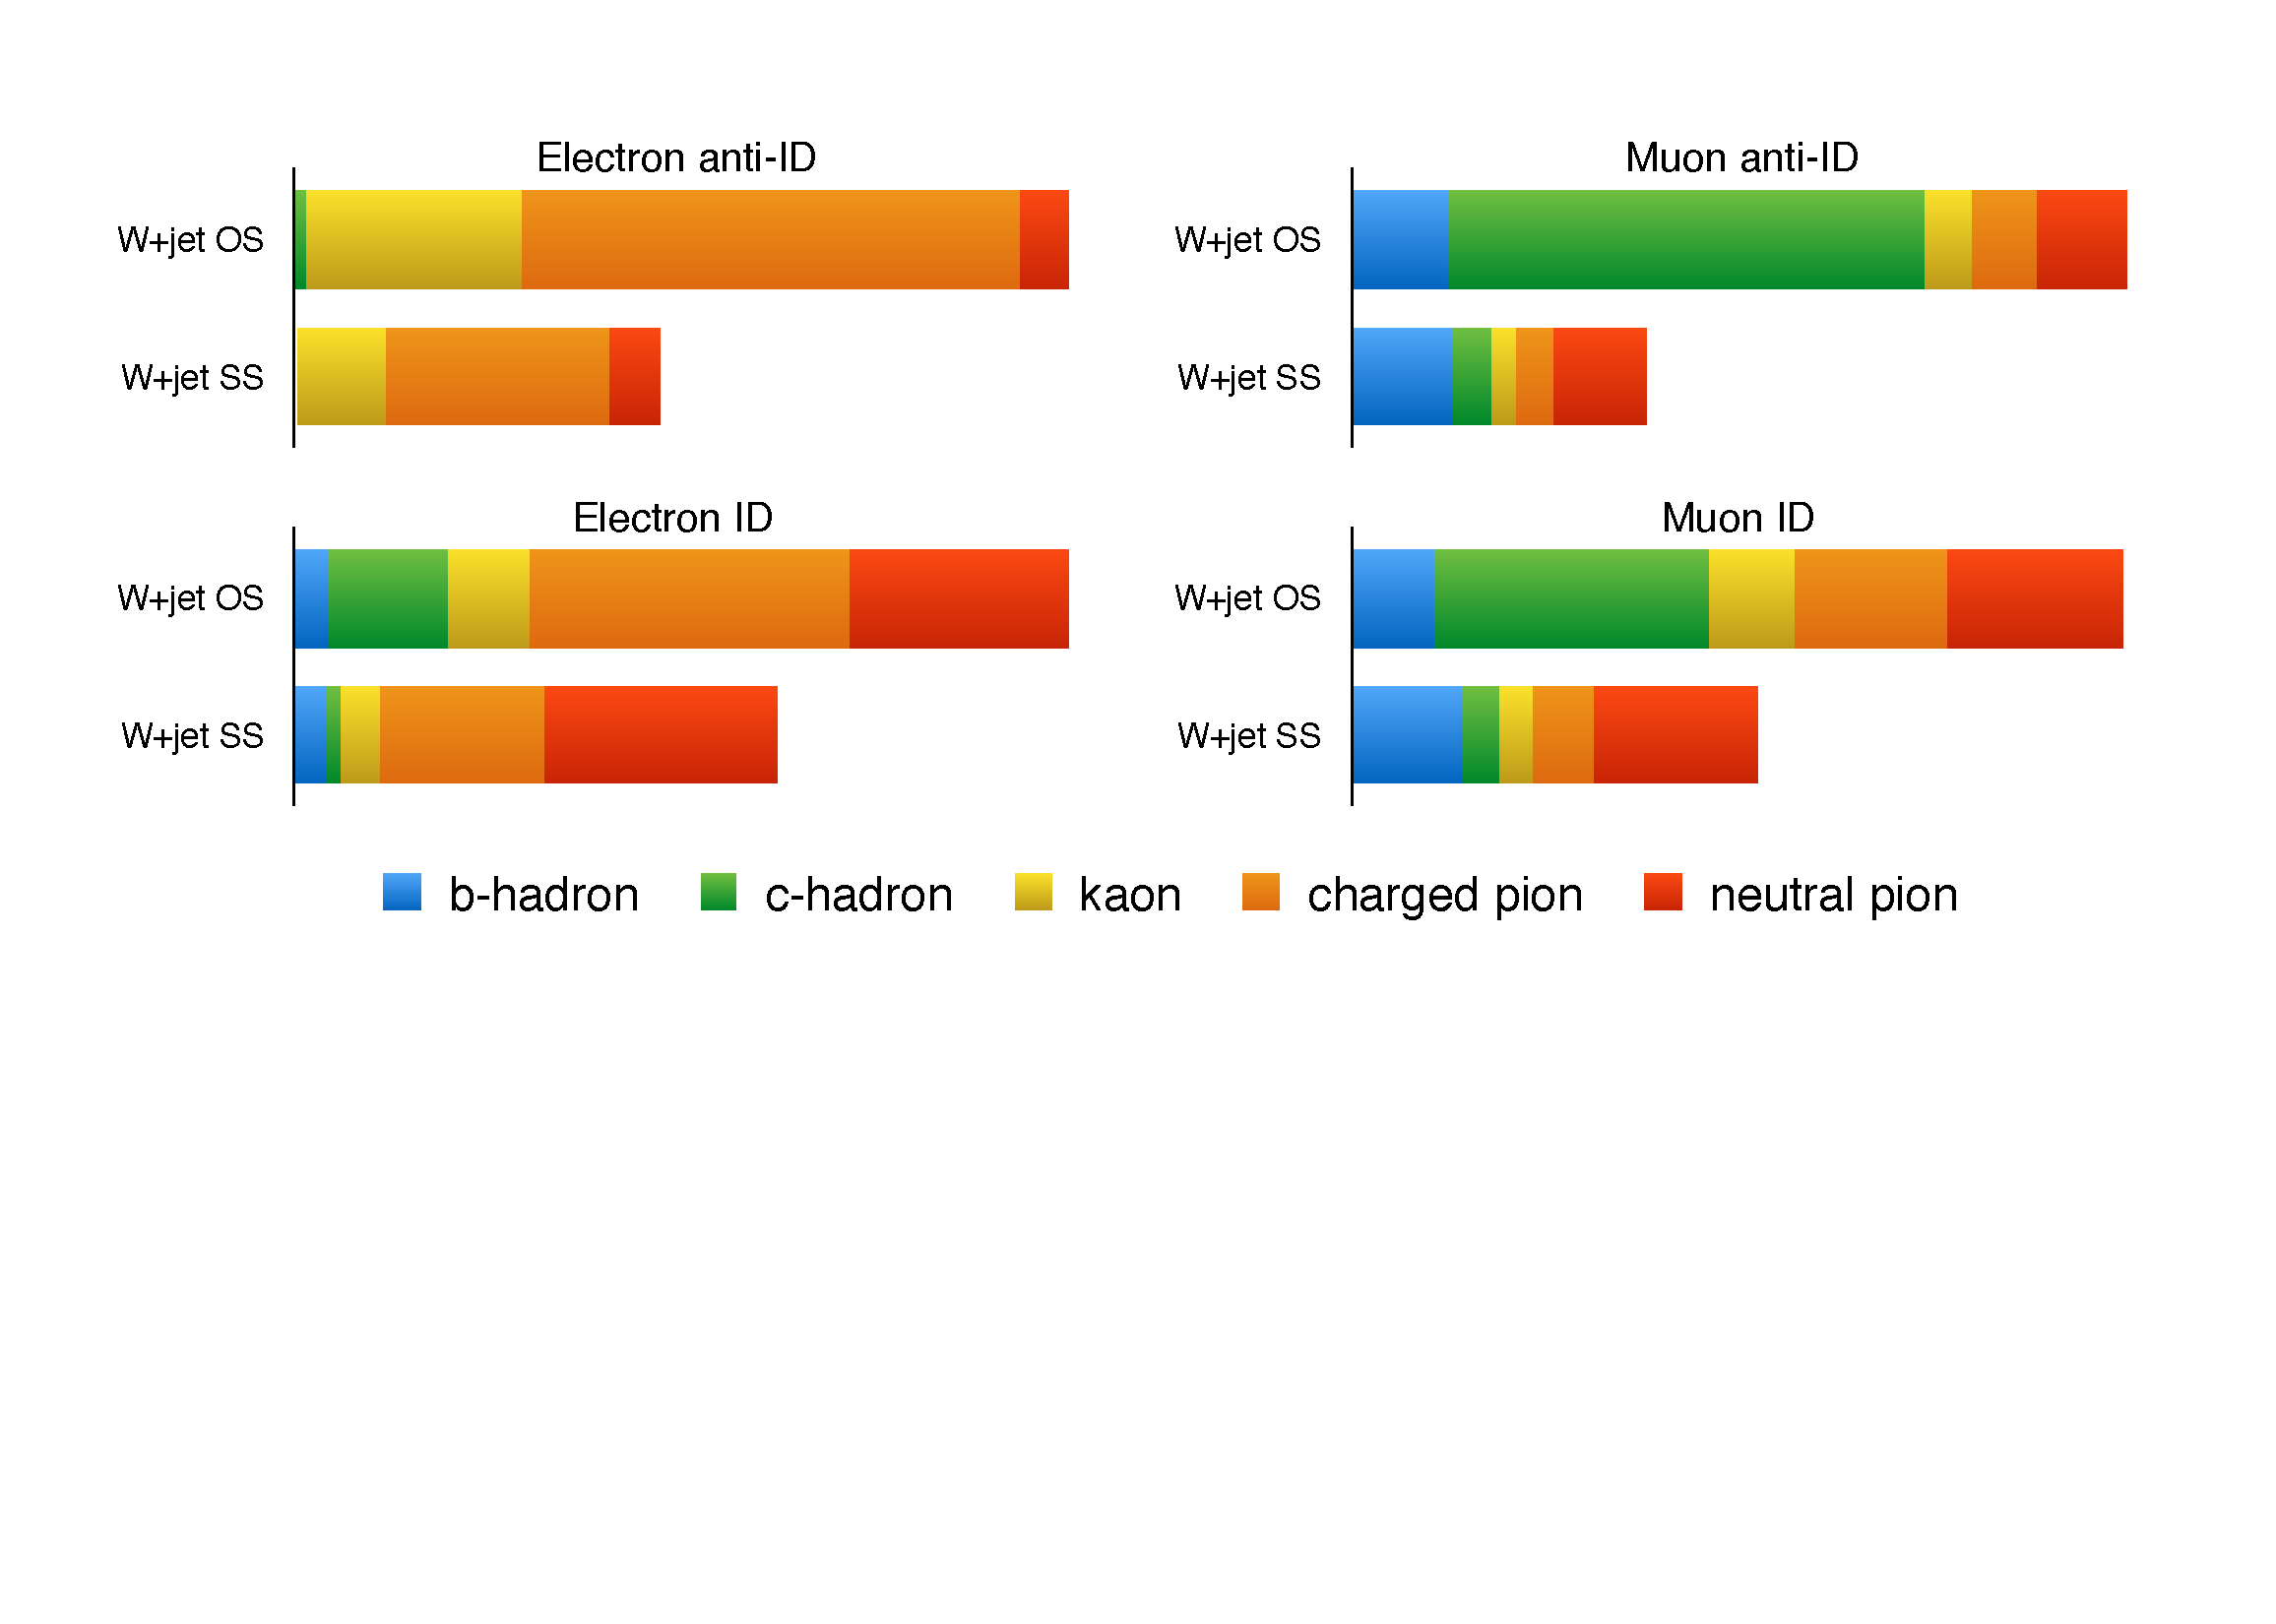
\includegraphics[width=\textwidth,clip=true,trim=1.8cm 12cm 2cm 2cm]{custom_images/wjets/wjets_flavcomp}
	\caption{The jet flavour composition of fake leptons, for opposite-sign (OS) and 
	same-sign (SS) \Wjets events. Each SS axis is scaled to the cross section of the 
	corresponding OS axis.}
	\label{fig:wjets:flav_comp}
\end{figure}

MC-based corrections are applied to the measured \Zjets fake factors in order to account 
for the different jet flavour compositions of the OS and SS \Wjets processes
\begin{equation}
	f_{\Plepton,i}^{\text{pred,\Wjets}}\parenths{\pt,\eta} &= f_{\Plepton}^{\text{data,\Zjets}}\parenths{\pt} \cdot \frac{f_{\Plepton}^{\text{data,dijet}}\parenths{\pt, \eta}}{f_{\Plepton}^{\text{data,dijet}}\parenths{\pt}} \cdot \frac{f_{\Plepton,i}^{\text{MC,\Wjets}}}{f_{\Plepton}^{\text{MC,\Zjets}}}
	\label{eq:wjet_ff}
\end{equation}
where $i = \text{OS, SS}$. The injection of $\eta$-dependence from the dijet fake factor 
is also shown in (\ref{eq:wjet_ff}). The \Zjets fake factor is used because \Zjets has a 
similar jet flavour composition to \Wjets. The correction factors are derived with 
\meps{\alpgen}{\pythia{6}}, and compared to those of \meps{\alpgen}{\fherwig} and 
\meps{\powhegbox}{\pythia{8}} to obtain a systematic uncertainty. The corrections factors 
are \statsyst{0.99}{0.05}{0.19} for OS electrons, \statsyst{1.00}{0.08}{0.21} for OS 
muons, \statsyst{1.25}{0.08}{0.30} for SS electrons and \statsyst{1.40}{0.14}{0.47} for 
SS muons.

The \Wjets background is dominated by uncertainties in the fake factor. These are split 
into components that are correlated and uncorrelated between 
$f_{\text{\Plepton,OS}}^{\text{\Wjets}}$ and $f_{\text{\Plepton,SS}}^{\text{\Wjets}}$. 
Components correlated between OS and SS largely cancel in the same-sign control region 
method of estimating the non-\WW diboson background (see \Section~\ref{sec:diboson:sscr}). 
This control region also offers validation of the \Wjets background estimation.



\subsection{Dijet background estimation}
\label{sec:wjets:dijet_bkg}

The dijet backgrounds to the dilepton and \Wjets samples are estimated from the dijet 
control sample, using (\ref{eq:dijet_bkgto_dilepton}) and (\ref{eq:dijet_bkgto_wjet}) 
respectively. The dijet control sample $\mathcal{N}_{\antiid{\Plepton}\antiid{\Plepton}}$ 
contains events with two anti-ID leptons, selected from events passing the data quality 
criteria and triggers specified in \Section~\ref{sec:selection}. They are accepted by the 
dilepton triggers since these have looser lepton selections. Contamination from \Wjets and 
other processes is estimated with MC, though is generally small.

The dijet fake factor $f_{\Plepton}^{\text{data,dijet}}$ is measured in events containing 
a balancing jet (passing the offline jet selection). However, in 
(\ref{eq:dijet_bkgto_dilepton}) and (\ref{eq:dijet_bkgto_wjet}) the fake factors are 
applied to events containing another anti-ID lepton 
($f_{\Plepton \vert \antiid{\Plepton}}^{\text{pred,dijet}}$), or as if there is an ID lepton
in the event ($f_{\Plepton \vert \id{\Plepton}}^{\text{pred,dijet}}$). This can heavily 
bias the jet flavour composition of the selected events, and this in turn can affect the 
fake factor of interest. For example, if the other object is a muon, this increases the 
probability that the event contains heavy flavour jets. Consequently, $f_{\Pe}$ would 
increase and $f_{\Pmu}$ would decrease (see \Section~\ref{sec:wjets:wjet_bkg}).

MC-based corrections are applied to the measured dijet fake factor in order to account 
for the correlation between $f_{\Plepton}$ and the other object in the event
\begin{equation}
	f_{\Plepton \vert \antiid{\Plepton}}^{\text{pred,dijet}}\parenths{\pt,\eta} &= f_{\Plepton}^{\text{data,dijet}}\parenths{\pt,\eta} \cdot \frac{f_{\Plepton \vert \antiid{\Plepton}}^{\text{MC,dijet}}}{f_{\Plepton \vert j}^{\text{MC,dijet}}} \\
	f_{\Plepton \vert \id{\Plepton}}^{\text{pred,dijet}}\parenths{\pt,\eta} &= f_{\Plepton}^{\text{data,dijet}}\parenths{\pt,\eta} \cdot \frac{f_{\Plepton \vert \id{\Plepton}}^{\text{MC,dijet}}}{f_{\Plepton \vert j}^{\text{MC,dijet}}} \,.
\end{equation}

The dijet background has a very small contribution to the \HWW signal regions, but has 
large uncertainties dominated by the MC-based corrections. It is difficult to define a 
high purity dijet validation region in the dilepton sample, though good agreement with 
experimental data is observed in the low \met regions where this background is enhanced.

